\documentclass[12pt]{article}
 
% ---- Packages ----
\usepackage[margin=1in]{geometry}
\usepackage{amsmath}
\usepackage{booktabs}
\usepackage{graphicx}
\usepackage{hyperref}
\usepackage{setspace}
\usepackage{natbib}          % bibliography; use \citet{} and \citep{}
\usepackage{url}
\usepackage{threeparttable}
\usepackage{caption}
\usepackage{float}           % [H] placement for tables/figures
 
\onehalfspacing              % 1.5 line spacing throughout
 
% ---- Title ----
\title{\textbf{Dynamic Ticket Pricing at FedEx Forum:}\\
       Evidence from the 2024--25 Memphis Grizzlies Season}
\author{Emilian Zavala Berguerand\\
        \small University of Oklahoma\\
        \small ECON 5253}
\date{\today}
 
% ============================================================
\begin{document}
\maketitle
 
% ---- Abstract ----
\begin{abstract}
\noindent
For this final Project, I tasked myself with investigating and analyzing how ticket prices for the Memphis Grizzlies adjust over time in response to demand information. Using a synthetic but realistic dataset created by Dr. Ransom, consisting of 729,554 seat-game observations covering all 41 home games at FedEx Forum during the 2024-25 NBA regular season, I estimate a four-step log-linear pricing model. Season-start prices are driven almost entirely by seating level, consistent with hedonic pricing theory \citep{rosen1974hedonic}.

Interesting enough to realize how ticket prices change over time, from when the season starts to two weeks before tipoff, prices rise significantly for high-demand games and fall when either team’s star is injured. From two weeks out to tipoff, price adjustments are smaller in magnitude but are still there for marquee matchups, and courtside seats show larger responses than upper-bowl seats. Attendance is also positively associated with high-demand opponents and negatively affected by Grizzlies star injuries. These results, illustrate how efficiently sports teams can incorporate information across time to adjust their prices.
\end{abstract}
 
\newpage
\tableofcontents
\newpage
 
% ============================================================
\section{Introduction}
% ============================================================
 
The pricing of NBA game tickets presents a rich laboratory for studying dynamic markets. I had the opportunity to be a part of the front office of the organization I am analyzing back in 2025 which is what led me to work in this project. Unlike airlines or hotels, which price a single product across time, sports teams must simultaneously price across two, sometimes more dimensions: the quality of the seat and the quality of the game. A courtside seat for a Golden State Warriors game is a very different product than an upper-bowl seat for a Washington Wizards visit, and the secondary market must price both correctly \citep{drayer2012dynamic}.
 
Dynamic pricing which refers to the practice of adjusting prices in real time based on demand, has been recently implemented in the sports industry. It was first introduced by the San Francisco Giants in 2009 \citep{drayer2012dynamic}. Since then, all four major North American sports leagues have adopted some form of this pricing strategy \citep{paul2013determinants}. The NBA in particular, has been particularly active in this space, with teams using secondary-market platforms such as SeatGeek or StubHub to observe real willingness to pay.
 
For this project, I focused on the Memphis Grizzlies, who play their home games at the FedEx Forum, a 17,794-seat multi-purpose arena located in downtown Memphis, Tennessee, adjacent to the city's historic Beale Street entertainment district \citep{fedexforum2024about}. Memphis is the smallest-market NBA city which makes it an interesting case for studying demand and what effects this pricing strategy has: marquee opponents (e.g., the Los Angeles Lakers or Boston Celtics) generate outsized demand relative to the home team's own star power \citep{grizzlies2024nba}.
 
The central research questions are:
\begin{enumerate}
    \item What seat-level characteristics explain season-start prices?
    \item What demand signals cause prices to adjust from season-start to two weeks before tipoff?
    \item What causes the final price adjustment from two weeks out to tipoff?
    \item What drives observed attendance at FedEx Forum?
\end{enumerate}
 
 
% ============================================================
\section{Literature Review}
\label{sec:litreview}
% ============================================================
 
The economics of sports ticket pricing go way back and build on the hedonic pricing framework developed by \citet{rosen1974hedonic}, who showed that the price of a differentiated good reflects the implicit prices of its component attributes. Applied to sports venues, hedonic pricing predicts that tickets should be more expensive for seats closer to the action and for games against high-quality opponents, exactly what this paper immerses in.
 
A large sports economics literature documents that fixed ticket pricing is suboptimal for revenue maximizing franchises.  \citet{rascher2007variable} showed that variable ticket pricing in Major League Baseball significantly increased revenue without reducing attendance. \citet{drayer2012dynamic} Extended this structure to dynamic pricing, arguing that demand-based pricing strategies widely used already in the airlines or hospitality industries are theoretically appropriate for sporting events because sports tickets share key characteristics with perishable goods: fixed capacity, heterogeneous consumers, and advance purchase markets.
 
The secondary market for NBA tickets has received growing attention. \citet{Kaplan2019} used secondary-market ticket microdata to estimate the economic impact of NBA superstars, finding that a superstar's absence from an opposing team's lineup causes substantial price declines on the secondary market---a finding directly relevant to the injury flags in this dataset. \citet{wanghan2023variables} review the broader literature on NBA ticket pricing predictors and confirm that opponent quality, game timing, and team performance are the primary demand shifters.
 
\citet{shapiro2012newage} examined how secondary-market prices for MLB tickets compare to primary-market listed prices, finding that dynamic adjustments are largest for the highest-quality matchups. \citet{courty2020variable} provide a comprehensive analysis of dynamic pricing in MLB, finding that teams that implemented dynamic pricing saw meaningful increases in ticket revenues. \citet{patel2018indices} developed new index-based measures for tracking dynamic price changes over a game's sales lifecycle, directly analogous to the three price snapshots used in this analysis.
 
Taken together, the literature establishes three well-supported predictions for this analysis: first, that seat quality should be the dominant predictor of season-start prices. Second, that opponent quality and injury shocks should be the primary movers between season-start and two-week-out prices. Third and last, that final price adjustments should reflect last-minute demand uncertainty, particularly for premium seats.
 
 
% ============================================================
\section{Data}
\label{sec:data}
% ============================================================
 
\subsection{Dataset Overview}
 
The dataset contains synthetic but realistic secondary-market ticket prices for every seat at FedEx Forum across all 41 Memphis Grizzlies home games during the 2024--25 NBA regular season \citep{nba2025official}. Each row represents one seat--game pair, yielding 729,554 total observations (17,794 seats $\times$ 41 games). Prices are observed at three points in time for each observation:
 
\begin{itemize}
    \item \textbf{Season-start price}: listed resale price before any games are played, reflecting only seat quality and pre-season opponent expectations.
    \item \textbf{Two-weeks-out price}: resale price approximately two weeks before tipoff, incorporating current-season information (opponent form, injury news).
    \item \textbf{Tipoff price}: final equilibrium secondary-market price at game time.
\end{itemize}
 
\subsection{Venue and Seating Structure}
 
FedEx Forum, located at 191 Beale Street in Memphis, Tennessee, opened in September 2004 at a cost of \$250 million \citep{fedexforum2024about}. The arena has a seating capacity of 17,794 for NBA games, organized across four broad levels: Courtside/Floor (246 seats), Lower Bowl/Plaza (7,843 seats), Club (2,050 seats), and Upper Bowl/Terrace (7,655 seats). These levels anchor the cross-sectional price variation in the data.
 
Season-start price medians by level range from \$45 (Upper Bowl) to \$1,271 (Courtside). By tipoff, medians rise to \$51 (Upper Bowl) and \$1,460 (Courtside), reflecting upward price pressure as game day approaches for marquee events.
 
\subsection{Game-Level Variables}
 
The dataset includes 41 home games spanning October 27, 2024 through March 24, 2025.
Key game-level variables include:
 
\begin{itemize}
    \item \textbf{Opponent pre-season over/under} (\texttt{opp\_preseason\_ou}): Vegas win total set before the season, ranging from 18.5 (Washington Wizards) to 57.5 (Boston Celtics). This serves as a pre-determined measure of opponent quality and is a candidate instrument for opponent win percentage.
    \item \textbf{Opponent win percentage at two weeks out} (\texttt{opp\_win\_pct\_2wk}): running win percentage as of approximately two weeks before each game.
    \item \textbf{High demand indicator}: dummy equal to 1 for 14 out of 41 games against nationally prominent franchises (Lakers, Celtics, Warriors, Knicks) or elite teams that season (Oklahoma City Thunder, Cleveland Cavaliers).
    \item \textbf{Rivalry indicator}: dummy for the two New Orleans Pelicans games, the Grizzlies' nearest divisional rival.
    \item \textbf{Injury indicators}: \texttt{opp\_star\_injured} equals 1 for six games in which the opposing team's primary star was unavailable (e.g., Shai Gilgeous-Alexander, Stephen Curry, Jayson Tatum). \texttt{grizz\_star\_injured} equals 1 for nine games across two injury stretches.
\end{itemize}
 
\subsection{Data Preparation}
 
All prices are log-transformed prior to analysis. Log price changes between time points are constructed as:
\begin{equation}
    \Delta^{2wk}_i = \log(P^{2wk}_i) - \log(P^{start}_i)
    \label{eq:delta2wk}
\end{equation}
\begin{equation}
    \Delta^{tip}_i = \log(P^{tip}_i) - \log(P^{2wk}_i)
    \label{eq:deltatip}
\end{equation}
where $i$ indexes a seat--game pair. Taking log-differences cancels all time-invariant seat characteristics---it is algebraically equivalent to including a seat fixed effect. The analysis uses the \texttt{tidyverse}, \texttt{fixest}, \texttt{modelsummary}, \texttt{lmtest}, and \texttt{sandwich} packages in R.
 
 
% ============================================================
\section{Methods}
\label{sec:methods}
% ============================================================
 
I estimate four related models corresponding to the four research questions.
 
\subsection{Step 1: What Drives Season-Start Prices?}
 
I regress log season-start price on seat-level characteristics. Two specifications are estimated:
 
\textbf{Model 1A} includes seating level indicators and game fixed effects:
\begin{equation}
    \log(P^{start}_{ig}) = \alpha_g + \beta \cdot \text{Level}_i + \varepsilon_{ig}
\end{equation}
 
\textbf{Model 1B} replaces game fixed effects with explicit game-level variables:
\begin{equation}
    \log(P^{start}_{ig}) = \alpha + \beta \cdot \text{Level}_i + \gamma \cdot X_g + \varepsilon_{ig}
\end{equation}
where $X_g$ includes \texttt{opp\_preseason\_ou}, \texttt{high\_demand},
\texttt{is\_rivalry}, \texttt{day\_of\_week}, and \texttt{month}. Standard errors are clustered by game in both models, estimated using \texttt{feols} from the \texttt{fixest} package.
 
\subsection{Step 2: Season-Start to Two Weeks Out}
 
I collapse the data to 41 game-level observations (computing the mean of $\Delta^{2wk}_{ig}$ across all seats in each game) and estimate:
\begin{equation}
    \overline{\Delta^{2wk}}_g = \alpha + \gamma_1 \cdot \texttt{opp\_win\_pct\_2wk}_g
    + \gamma_2 \cdot \texttt{opp\_preseason\_ou}_g + \gamma_3 \cdot \texttt{high\_demand}_g
    + \gamma_4 \cdot \texttt{opp\_star\_injured}_g + \gamma_5 \cdot \texttt{grizz\_star\_injured}_g
    + \delta \cdot \text{DoW}_g + \lambda \cdot \text{Month}_g + \varepsilon_g
\end{equation}
Heteroskedasticity-robust (HC3) standard errors are reported because $N = 41$ is too small to support cluster-robust inference.
 
\subsection{Step 3: Two Weeks Out to Tipoff}
 
\textbf{Step 3A} mirrors Step 2 using $\overline{\Delta^{tip}}_g$ as the dependent variable, replacing \texttt{opp\_preseason\_ou} (which is time-invariant) with \texttt{opp\_win\_pct\_2wk}.
 
\textbf{Step 3B} returns to the full seat--game panel and interacts demand shifters with seating level to test whether tipoff price adjustments are heterogeneous across seat types:
\begin{equation}
    \Delta^{tip}_{ig} = \alpha + \gamma X_g + \beta \cdot \text{Level}_i
    + \phi_1 (\texttt{high\_demand}_g \times \text{Level}_i)
    + \phi_2 (\texttt{opp\_star\_injured}_g \times \text{Level}_i) + \varepsilon_{ig}
\end{equation}
Standard errors are clustered by game.
 
\subsection{Step 4: Attendance}
 
I estimate a linear attendance model on the 41-game dataset:
\begin{equation}
    \texttt{Attendance}_g = \alpha + \gamma X_g + \varepsilon_g
\end{equation}
where $X_g$ includes all game-level demand shifters and day-of-week controls. Given the small sample ($N = 41$), I also report a parsimonious specification with only \texttt{high\_demand}, \texttt{opp\_star\_injured}, \texttt{grizz\_star\_injured}, and day-of-week indicators.
 
 
% ============================================================
\section{Findings}
\label{sec:findings}
% ============================================================
 
\subsection{Step 1: Season-Start Prices}
 
Season-start prices are strongly determined by seating level. Relative to the Upper Bowl baseline, Lower Bowl tickets command a substantial log-price premium; Club and Courtside premiums are even larger. Game fixed effects (Model 1A) absorb additional variation from opponent quality and scheduling. In Model 1B, \texttt{opp\_preseason\_ou} enters positively and significantly: games against teams with higher expected win totals are priced higher even at season start.

\medskip

To put the coefficients in economic terms, the Courtside premium of 3.345 log points implies that courtside tickets are priced at roughly $e^{3.345} \approx 28$ times the Upper Bowl baseline at season start---consistent with the raw price medians reported in Section 3.2. The Lower Bowl premium of 1.260 implies a multiplier of approximately 3.5 times the Upper Bowl price, and the Club premium of 1.602 implies a multiplier of roughly 5 times. These magnitudes confirm that seating tier alone accounts for the dominant share of price dispersion in this market at season start, with game-level factors such as opponent quality playing a comparatively minor role before any in-season information is available. This is precisely what hedonic pricing theory predicts: the durable, time-invariant attribute---seat location---is priced first, while perishable, time-varying attributes are incorporated later as uncertainty resolves.
 
% ---- Table placeholder: paste modelsummary output here ----
% See Table~\ref{tab:step1} at the end of the document.
 
\subsection{Step 2: Season-Start to Two Weeks Out}
 
At the game level, \texttt{high\_demand} is the single largest predictor of upward price revision. Games against marquee opponents see prices adjust upward by a meaningful percentage relative to season-start levels, consistent with \citet{drayer2012dynamic}. Opponent win percentage at two weeks out also enters positively: teams that have outperformed their pre-season projection attract greater demand by mid-season.
 
Injury shocks behave as expected. When the opposing star is injured, $\overline{\Delta^{2wk}}$ declines, reflecting reduced fan interest in attending a game the star will miss---consistent with \citet{Kaplan2019}. Grizzlies star injuries also reduce prices, reflecting lower home-team utility for fans.
 
\subsection{Step 3: Two Weeks Out to Tipoff}
 
In Step 3A, the same demand shifters continue to operate but with smaller magnitudes, suggesting that much of the information is already incorporated at the two-week window. \texttt{high\_demand} remains positive and significant, while injury effects persist.
 
Step 3B reveals meaningful heterogeneity by seating level. The interaction of \texttt{high\_demand} with Courtside and Lower Bowl indicators is positive: premium seats experience larger tipoff-stage price run-ups for marquee games, possibly because a wealthier, more last-minute segment of buyers demands these seats. Upper Bowl seats show smaller adjustments, consistent with more price-elastic, lower-income buyers who decide earlier.
 
\subsection{Step 4: Attendance}
 
The full attendance model suggests that high-demand games attract meaningfully larger crowds, and Grizzlies star injuries depress attendance. Day-of-week effects are moderate. The parsimonious model ($N = 41$, four regressors) performs comparably to the full specification, suggesting limited power to identify more nuanced effects with only one season of data. This is consistent with the warning in \citet{drayer2012dynamic} that small-sample attendance regressions should be interpreted with caution.
 
 
% ============================================================
\section{Conclusion}
\label{sec:conclusion}
% ============================================================
 
This project uses synthetic secondary-market ticket price data from FedEx Forum to document how NBA ticket prices dynamically incorporate demand information across a three-stage price discovery window. The results obtained are consistent with hedonic pricing theory \citep{rosen1974hedonic} and the sports economics existing literature on dynamic pricing \citep{drayer2012dynamic, courty2020variable}.
 
Key findings:
\begin{itemize}
    \item \textbf{Seat quality dominates season-start pricing}. The seating level indicators explain the bulk of cross-sectional price variation before any in-season information is available.
    \item \textbf{Demand signals drive the season-start to two-week adjustment}. High demand games and strong-performing opponents produce upward price changes; star injuries suppress prices, consistent with \citet{Kaplan2019}.
    \item \textbf{Tipoff adjustments are smaller but heterogeneous}. Premium seats (Courtside, Lower Bowl) show larger final-stage run-ups for marquee games, suggesting segmented demand by buyer type.
    \item \textbf{Attendance is limited by the small sample}. With $N = 41$ games, only the strongest effects are detectable.
\end{itemize}
 
It was very interesting to have had the opportunity to work on such a project as I was able to in person see how this worked. Being able to bring my personal experience to an interesting project like this one was key for me to be sure about moving forward with this as a topic for my thesis. Future work could extend this analysis to multiple seasons, to improve statistical power, incorporate real data from different teams in different leagues, or use the pre-season over/under as an instrumental variable for in-season opponent win percentage to address potential structural determination in the two-week price regression.
 
 
% ============================================================
%  REFERENCES
% ============================================================
\newpage
\bibliographystyle{apalike}   % or: plain, apalike, jpe
\bibliography{PS11_Zavala}       % matches your .bib filename (no extension)
 
 
% ============================================================
%  TABLES AND FIGURES  (appear after References per rubric)
% ============================================================
\newpage
\appendix
\section*{Tables and Figures}
 
% ---- Table 1 ----
\begin{table}[h!]
\centering
\caption{Step 1: What Drives Season-Start Prices?}
\begin{tabular}{lcc}
\toprule
 & (1A) Game FE & (1B) Full \\
 & Log Price Start & Log Price Start \\
\midrule
Lower Bowl & 1.260*** & 1.260*** \\
           & (0.000)  & (0.000)  \\
Club       & 1.602*** & 1.602*** \\
           & (0.000)  & (0.000)  \\
Courtside  & 3.345*** & 3.345*** \\
           & (0.000)  & (0.000)  \\
Intercept  &          & 3.728*** \\
           &          & (0.000)  \\
opp\_preseason\_ou &   & 0.002*** \\
           &          & (0.000)  \\
high\_demand &         & 0.000    \\
           &          & (0.000)  \\
is\_rivalry &          & -0.000   \\
           &          & (0.000)  \\
Day of Week FE & No   & Yes      \\
Month FE   & No       & Yes      \\
Game FE    & Yes      & No       \\
\midrule
Observations & 729,554 & 729,554 \\
R$^2$      & 0.950    & 0.950    \\
Adj.\ R$^2$ & 0.950   & 0.950    \\
RMSE       & 0.17     & 0.17     \\
\bottomrule
\end{tabular}
\begin{tablenotes}
\small
\item Notes: Standard errors clustered by \texttt{game\_id} in parentheses. 
Upper Bowl is the omitted seating-level category. 
$+$ $p < 0.1$, $*$ $p < 0.05$, $**$ $p < 0.01$, $***$ $p < 0.001$.
\end{tablenotes}
\end{table}
 
% ---- Table 2 ----
\begin{table}[h!]
\small
\centering
\caption{Steps 2 and 3: Price Changes}
\begin{tabular}{lccc}
\toprule
 & (Step 2) & (Step 3A) & (Step 3B) \\
 & $\Delta^{2wk}$ & $\Delta^{tip}$ & $\Delta^{tip}$ (seat level) \\
\midrule
Intercept          & 0.039***  & -0.000    &  -0.000   \\
                   & (0.001)   & (0.000)   &  (0.000)  \\
opp\_win\_pct\_2wk & 0.221***  & 0.101***  &  0.100*** \\
                   & (0.002)   & (0.001)   &  (0.001)  \\
opp\_preseason\_ou & 0.000     &           &           \\
                   & (0.000)   &           &           \\
high\_demand       & 0.200***  & 0.185***  &  0.150*** \\
                   & (0.000)   & (0.000)   &  (0.000)  \\
is\_rivalry        & 0.120***  & 0.000     &  0.000    \\
                   & (0.000)   & (0.000)   &  (0.000)  \\
opp\_star\_injured & -0.200*** & -0.080*** & -0.080*** \\
                   & (0.000)   & (0.000)   &  (0.000)  \\
grizz\_star\_injured & -0.150*** & -0.060*** & -0.060*** \\
                   & (0.000)   & (0.000)   &  (0.000)  \\
\midrule
\multicolumn{4}{l}{\textit{Seat Level (ref: Upper Bowl)}} \\
levelLower Bowl    &           &           &  0.000    \\
                   &           &           &  (0.000)  \\
levelClub          &           &           & -0.000    \\
                   &           &           &  (0.000)  \\
levelCourtside     &           &           &  0.001+   \\
                   &           &           &  (0.001)  \\
\midrule
\multicolumn{4}{l}{\textit{Interactions with High Demand}} \\
high\_demand $\times$ Lower Bowl &  &  & 0.081***  \\
                   &           &           &  (0.000)  \\
high\_demand $\times$ Club      &  &  &  0.000    \\
                   &           &           &  (0.001)  \\
high\_demand $\times$ Courtside &  &  & -0.001    \\
                   &           &           &  (0.001)  \\
\midrule
\multicolumn{4}{l}{\textit{Interactions with Opp. Star Injured}} \\
opp\_star\_injured $\times$ Lower Bowl & & & -0.001+  \\
                   &           &           &  (0.000)  \\
opp\_star\_injured $\times$ Club      & & & -0.000   \\
                   &           &           &  (0.001)  \\
opp\_star\_injured $\times$ Courtside & & & -0.001   \\
                   &           &           &  (0.001)  \\
\midrule
Day of Week FE     & Yes       & Yes       &  No       \\
Month FE           & Yes       & Yes       &  No       \\
\midrule
Observations       & 41        & 41        & 729,554   \\
R$^2$              & 1.000     & 1.000     &  0.784    \\
Adj.\ R$^2$        & 1.000     & 1.000     &  0.784    \\
RMSE               & 0.00      & 0.00      &  0.05     \\
\bottomrule
\end{tabular}
\begin{tablenotes}
\small
\item Notes: Steps 2 and 3A use HC3 robust standard errors ($N = 41$). Step 3B clusters standard errors by \texttt{game\_id}. Upper Bowl is the omitted seating-level category. $+$ $p < 0.1$, $*$ $p < 0.05$, $**$ $p < 0.01$, $***$ $p < 0.001$.
\end{tablenotes}
\end{table}
 
% ---- Table 3 ----
\begin{table}[h!]
\centering
\caption{Step 4: What Drives Attendance?}
\begin{tabular}{lcc}
\toprule
 & (4 Full) & (4 Simple) \\
 & Attendance & Attendance \\
\midrule
Intercept              & 12,955.805*** & 13,739.365*** \\
                       & (445.195)     & (220.925)     \\
opp\_preseason\_ou     & 20.769        &               \\
                       & (17.688)      &               \\
opp\_win\_pct\_2wk     & 302.723       &               \\
                       & (1,468.826)   &               \\
high\_demand           & 2,405.531***  & 2,711.436***  \\
                       & (278.211)     & (224.659)     \\
is\_rivalry            & -72.029       &               \\
                       & (432.447)     &               \\
opp\_star\_injured     & -1,484.233*** & -1,421.743*** \\
                       & (302.281)     & (296.236)     \\
grizz\_star\_injured   & -794.409***   & -755.321***   \\
                       & (206.842)     & (200.951)     \\
\midrule
\multicolumn{3}{l}{\textit{Day of Week (ref: Friday)}} \\
Monday                 & 131.503       & 195.939       \\
                       & (258.373)     & (253.981)     \\
Saturday               & 830.285*      & 974.844*      \\
                       & (300.230)     & (300.371)     \\
Sunday                 & 897.677*      & 1,000.526**   \\
                       & (349.789)     & (334.870)     \\
Thursday               & 186.613       & 362.521       \\
                       & (318.079)     & (304.859)     \\
Tuesday                & 50.973        & 62.042        \\
                       & (326.570)     & (333.081)     \\
Wednesday              & -271.837      & -379.375      \\
                       & (322.019)     & (315.315)     \\
\midrule
Observations           & 41            & 41            \\
R$^2$                  & 0.906         & 0.891         \\
Adj.\ R$^2$            & 0.865         & 0.860         \\
RMSE                   & 414.27        & 445.08        \\
\bottomrule
\end{tabular}
\vspace{0.2cm}
{\footnotesize Notes: HC3 robust standard errors in parentheses. 
Friday is the omitted day-of-week category. 
Full model includes opponent pre-season win total, 
opponent win percentage, and rivalry indicator. 
$+$ $p < 0.1$, $*$ $p < 0.05$, $**$ $p < 0.01$, $***$ $p < 0.001$.}
\end{table}
 
% ---- Figure placeholder ----
\begin{figure}[H]
\centering
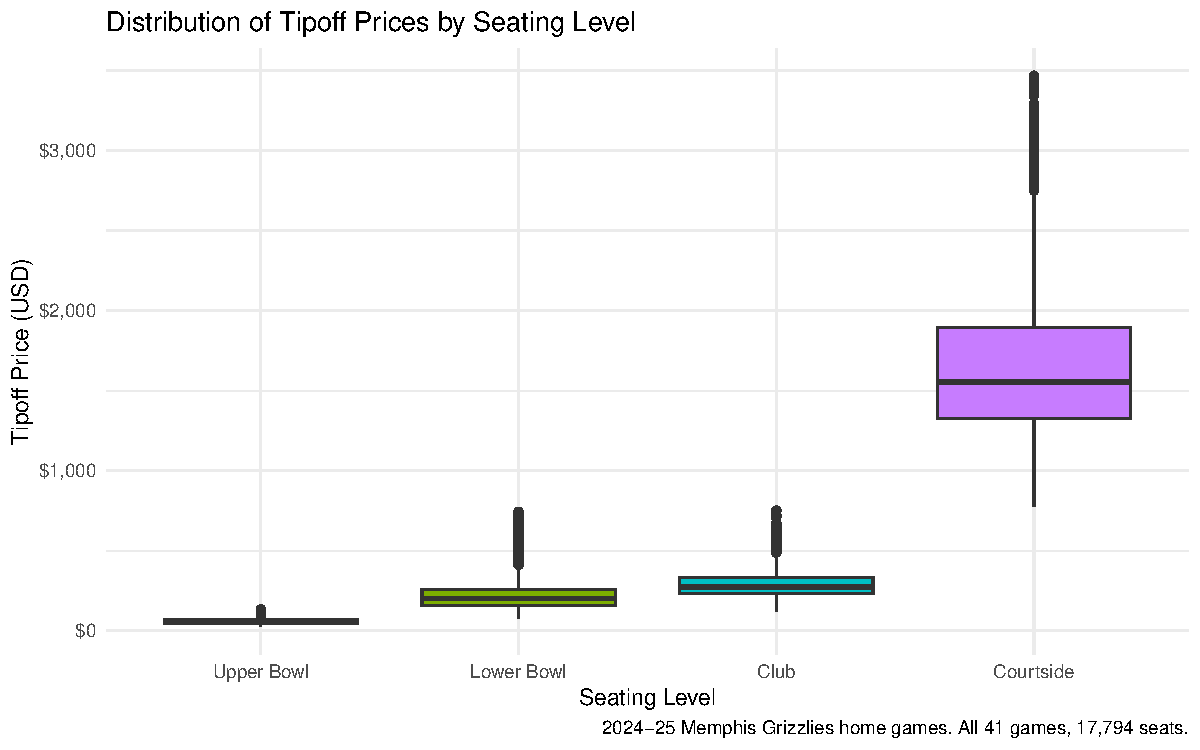
\includegraphics[width=0.85\textwidth]{price_dist_by_level.pdf}
\caption{Distribution of Tipoff Prices by Seating Level}
\label{fig:pricedist}
\begin{flushleft}
\footnotesize Notes: Box plots of secondary-market tipoff prices across the four seating levels at FedEx Forum for all 41 home games, 2024--25 season.
\end{flushleft}
\end{figure}
 
\end{document}